\chapter{Design and Methodology}
Chapter Three provides a detailed description of the design decisions for the research, building on the foundations and stemming from the related work reviewed in Chapter Two. Firstly, a set of requirements are gathered to ensure that the research objectives and challenges outlined in Chapter One are met. Subsequent sections then present the design solution and provide a discussion of the implications of the decisions made during the design process.
\section{Data Gathering}
\subsection{IIT Bombay English-Hindi Parallel Corpus}
IIT Bombay English-Hindi Parallel Corpus was presented by Kunchukuttan et al. The corpus is a compilation of parallel corpora which was previously available in the public domain as well as the new corpus they collected.Currently there is unavailability of large parallel corpus in Hindi-English containing multi-domain data, which is very necessary for neural machine translation.The decision to use IIT-Bombay English-Hindi Parallel Corpus was due its large size and quality of data it contains. It is the largest publicly available English-Hindi parallel corpus and was presented in 11th edition of the Language Resources and Evaluation Conference 2018. The corpus contains 1.49 million parallel sentence segments of which 694K segments are newly collected and not previously available in the public domain, which makes it perfect fit for this neural machine translation task. 

The parallel corpus has been compiled form a variety of existing sources like OPUS (Tiedemann, 2012), HindEn (Bojar et al., 2014b) and TED (Abdelali et al., 2014)) as well as the corpora developed at the Centre for Indian Language Technology, IIT Bombay over the years. The training corpus is consisted of sentences, phrases , dictionary entries spanning across multiple applications and domains. The details of the training set have been shown in Table 3.1.

\subsubsection{Corpus Details}
The details of the new sub-corpora that was added to the collection for the IIT Bombay English-Hindi Parallel Corpus are as follows.

\textbf{Judicial domain corpus - I} contains translations of legal judgments by in-house translators with many years with many years of translation experience though they didn’t have knowledge of the legal domain.

\textbf{Judicial domain corpus - II} contains translation done by graduate student who took part in a graduate course on natural language processing. This exercise was part of collecting translation in a complex domain by non-expert translators. The translations included in the corpus were determined to be of good quality by annotators.

\textbf{Mahashabdkosh 2} is an online official terminology dictionary website which is hosted by Department of Official Language, India. It contains Hindi and its equivalent English definitions. The translation sentence pairs were crawled from the official website.

\textbf{Indian Government corpora} was manually collected by the staff form Center for Indian Language Technology from various government websites like the National Portal of India, Reserve Bank of India, Ministry of Human Resource Development, NABARD,etc.

\textbf{Hindi-English Linked Wordnet} contains bilingual dictionary entries created from the linked Hindi and English wordnets.

\textbf{Gyaan-Nidhi Corpus} is a million pages multilingual parallel text corpus in English and 11 Indian languages (Assamese, Bengali, Gujarati, Hindi, Kannada, Marathi, Malayalam, Oriya, Punjabi, Tamil \& Telugu) based on Unicode encoding. The authors performed sentence alignment technique proposed by Moore (2002) to extract the parallel corpora from this comparable corpora. 

\begin{table}[h]
\centering
\resizebox{\textwidth}{!}{\begin{tabular}{rrr}
  \hline \textbf{Corpus Id} & \textbf{Source} & \textbf{Number of Segments} \\ 
  \hline
  1&GNOME (OPUS) (Tiedemann, 2012))&145,706\\
  2&KDE4 (OPUS) &97,227\\
  3&Tanzil (OPUS)&187,080\\
  4&Tatoeba (OPUS)&4,698\\
  5& OpenSubs2013 (OPUS)&4,222\\
  6& HindEnCorp (Bojar et al., 2014b)&273,885\\
  7&Hindi-English Linked Wordnets (Bhattacharyya, 2010)& 175,175\\
  8&Mahashabdkosh: Administrative Domain Dictionary
(Kunchukuttan et al., 2013)&66,474\\
9&Mahashabdkosh: Administrative Domain Examples &46,825\\
10& Mahashabdkosh: Administrative Domain Definitions&46,523\\
11&TED talks (Abdelali et al., 2014) &42,583\\
12&Indic Multi-parallel corpus (Alexandra Birch and Post, 2011)&10,349\\
13&Judicial domain corpus - I (Kunchukuttan et al., 2013)&5,007\\
14&Judicial domain corpus - II (Kunchukuttan et al., 2012)&3,727\\
15&Indian Government corpora&123,360\\
16&Wiki Headlines (Provided by CMU: www.statmt.org/wmt14/wiki-titles.tgz)&32,863\\
17& Gyaan-Nidhi Corpus &227,123\\
\hline
\textbf{Total}&&\textbf{1,492,827}\\
\hline
\end{tabular}}
\caption{Details of the IITB English-Hindi Parallel Corpus (training set)}
\end{table}

\subsubsection{Corpus Statistics}
The test and dev corpora used in the IIT Bombay Hindi-English Corpus are the same ones that was used for the WMT 2014 English-Hindi shared task (Bojar et al., 2014a) which contains newswire sentences. The detailed statistics about the whole dataset is shown in Table 3.3.

\begin{table}[h!]
\centering
 \begin{tabular}{ |ccc| } 
  \hline \textbf{Set} & \textbf{Description} & \textbf{Number of Segments}  \\ 
  \hline
  Dev (use for tuning)& Newswire (from WMT 2014)&520\\
  Test (use for final evaluation)& Newswire (from WMT 2014) &2507\\
  \hline
 \end{tabular}
\caption{Details of the IITB English-Hindi Parallel Corpus (Dev and Test set)}
\end{table}

\begin{table}[h!]
\centering
 \begin{tabular}{ |ccccc| } 
  \hline &\textbf{Language} & \textbf{Train} & \textbf{Test} & \textbf{Dev} \\ 
  \hline 
  \#Sentences && 1,492,827&2,507& 520\\
  \hline
  \#Tokens& eng&20,667,259 &57,803& 10,656\\
  &hin& 22,171,543&63,853&10,174\\
  \hline
  \#Types&eng&250,782&8,957& 2,569\\
  &hin& 343,601&8,489& 2,625\\
  \hline
 \end{tabular}
\caption{Statistics of data sets}
\end{table}

\subsubsection{Corpus Quality}
The IIT Bombay Hindi-English Parallel Corpus contains about 1.49 million Hindi – English sentence pairs which is an excellent fit for Neural Machine Translation. Though the Neural Machine Translation models demand much larger parallel corpora for better performance, but this corpus  is sufficient to train an efficient model. This corpus achieved the benchmark on baseline SMT and NMT systems. This corpus was also used for the three shared tasks (Workshop on Asian Language Translation 2016, 2017 and 2018). The quality of corpus also depends on its content, the data in this corpus is collected from multiple domains which makes it fitter for neural machine translation. The corpus contains data from domains such as Judicial , Health , Tourism , Administrative etc making it more apt for creating a generic neural translation model which works efficiently irrespective of domain.
All the data (training, dev and text) in the parallel corpus is normalized and tokenized which makes it easier for training neural translation models. For Hindi, the Indic NLP library by Kunchukuttan was used , whereas for English the Moses tokenizer was used.  




\subsection{Domain specific Corpus Generation for Fine Tuning}


\section{Neural Translation Model}

\begin{figure}
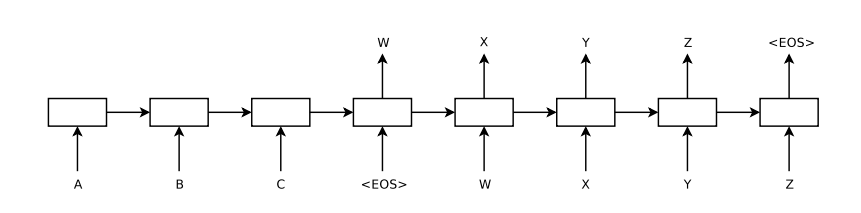
\includegraphics[width=\textwidth]{figures/nmt1.png}
\caption{Sequence to Sequence Learning with Neural Networks} \label{fig1}
\end{figure}
\section{Visual Interface}